% TEMP
\pagebreak

\subsection{Korrektur der Texturen}

Vor der Greedy Meshing Implementation sah eine
typische Spielwelt so aus:

\begin{center}
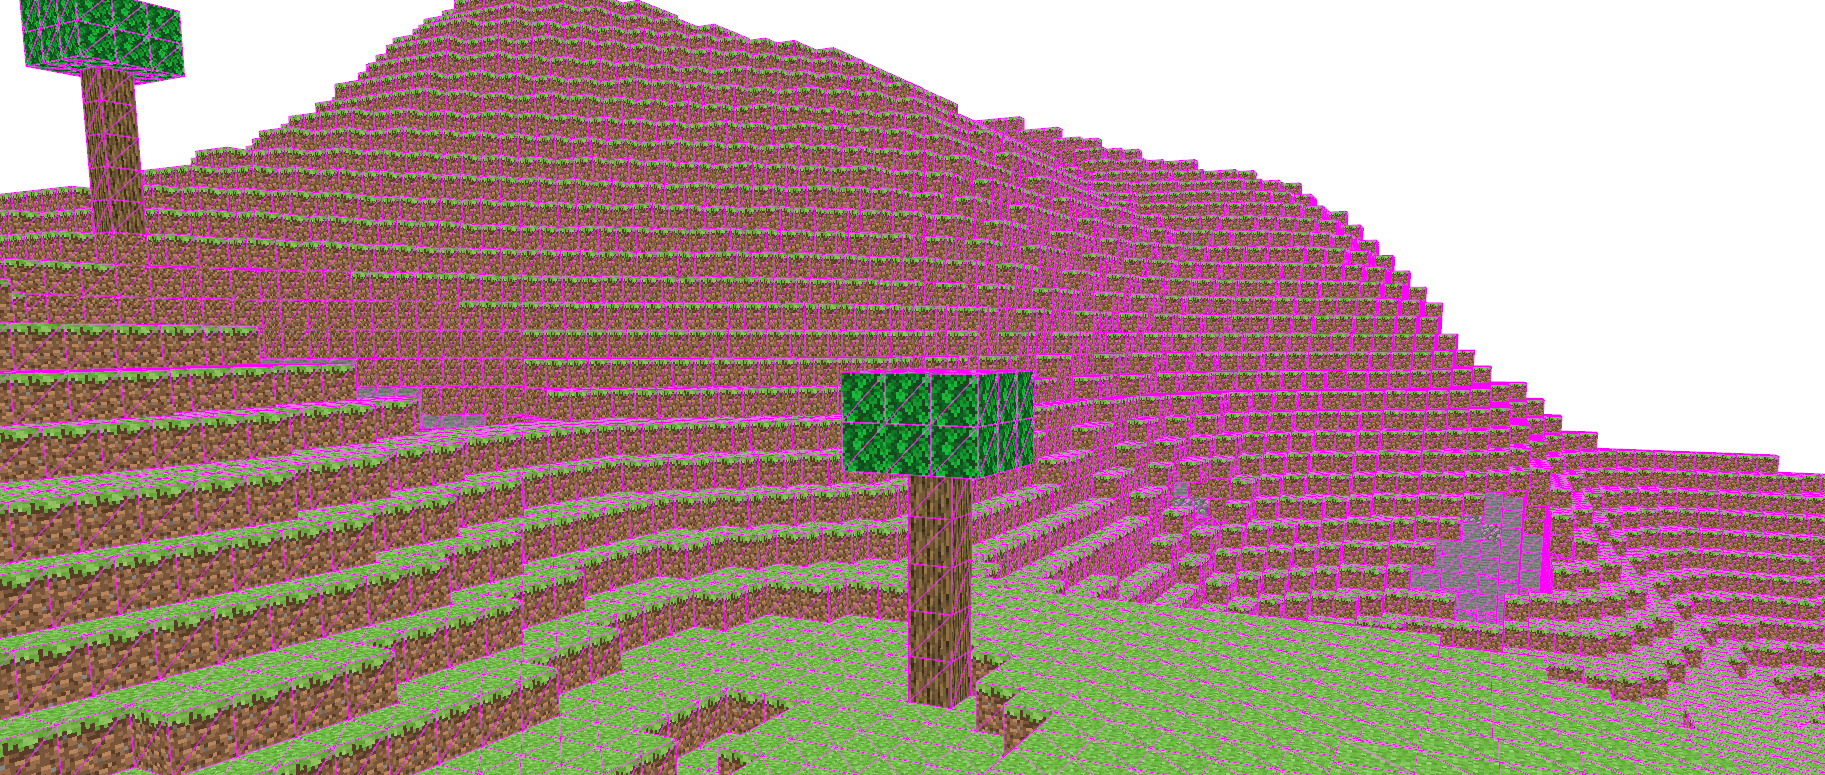
\includegraphics[width=0.8\textwidth]{../assets/greedy/landscape_normal.png}
\end{center}

Aber jetzt mit der neuen Implementation
sieht die gleiche Spielwelt wie folgt aus:

\begin{center}
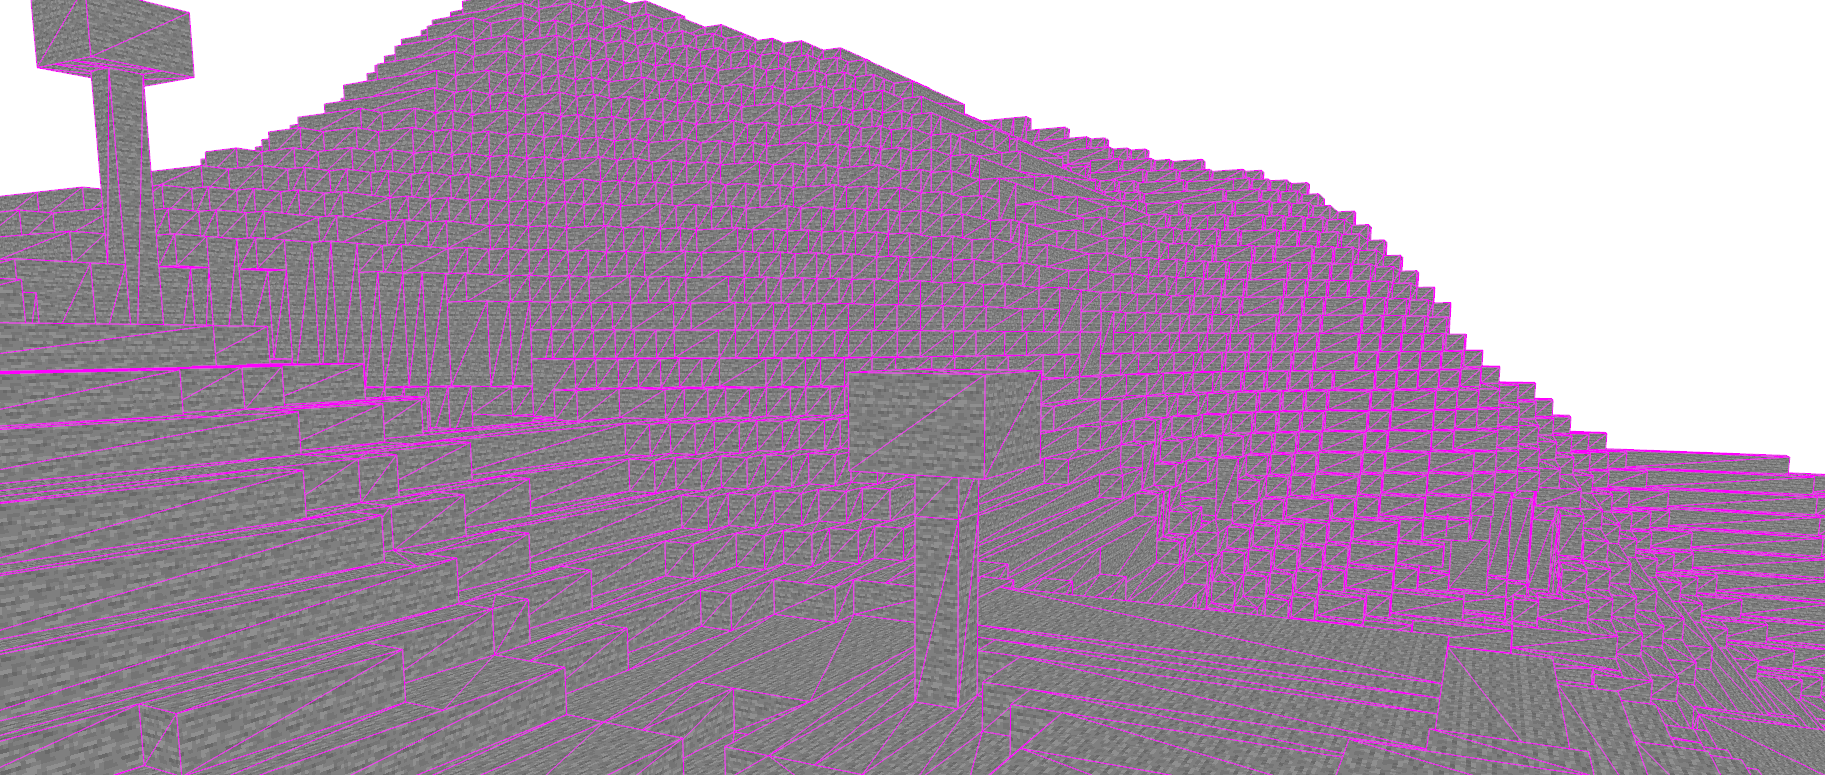
\includegraphics[width=0.8\textwidth]{../assets/greedy/landscape_stone_only.png}
\end{center}

Das Problem ist, dass wir noch nicht überlegt haben,
wie die Texturen der Voxels in das Polygonnetz des
Chunks eingebaut werden.
Bevor wir Greedy Meshing benutzt haben, konnte man
einfach jedem Dreieck eine Textur geben, basierend
darauf zu welchem Voxel es gehört.
Jedoch kann jetzt ein Dreieck für mehrere Voxels
zuständig sein.

In \cite{yt_bin_greedy_mesher} und
\cite{gh_bin_greedy_mesher} wurden hierfür separate
Polygonnetze und Bitmasken für jede Art von Voxel
verwendet (und es gab auch keine Texturen, sondern
nur Farben).
In meinem Spiel will ich jedoch viele unterschiedliche
Arten von Voxels haben. Deswegen wäre es unrealistisch
ein separates Polygonnetz für jede Art zu haben.
Meine Strategie um dieses Problem zu lösen ist es,
mehrere Texturen auf einem Dreieck anzuzeigen.

% if this is a bad place for a \pagebreak,
% then insert some \vspace here
\pagebreak

Um dies zu verstehen, müssen wir erst einmal angucken,
wie die Texturen in einem Polygonnetz ohne
Greedy Meshing angewandt werden.
Es wird erst ein Array von Texturen erstellt,
das alle möglichen Texturen von Voxels beinhaltet.
Beim Erstellen des Polygonnetzes bekommt
dann jedes Dreieck\footnote{
	In Wirklichkeit kann man mit WebGPU nicht
	Daten mit jedem Dreieck assoziieren,
	sondern nur mit jedem Vertex.
	Somit speichern wir diesen Index doppelt so
	oft, wie wir es brauchen.
	Aber es geht hier um nur sehr wenig Daten,
	also ist das nicht relevant.
}
in dem Polygonnetz einen Index,
den es benutzen kann, um die richtige Textur für
dieses Voxel in dem Array zu finden.

Die einfachste Lösung wäre also, anstatt nur
einen Index zu speichern, ein 2 dimensionales Array
von Indexen zu speichern für jeden Voxel,
der von diesem Dreieck dargestellt wird.
Leider geht dies nicht, da alle Informationen,
die man für einzelne Dreiecke (also nicht das
gesamte Polygonnetz) speichern will, müssen in dem
\href{https://gpuweb.github.io/gpuweb/#enumdef-gpuvertexformat}{\code{GPUVertexFormat}}\cite{gpu_vertex_format}
sein.
Dabei gibt es nur Datentypen mit konstanter Größe,
wir brauchen aber ein Array mit dynamischer Länge.
Zudem wäre es unrealistisch immer das größtmögliche
Array zu speichern und unbenutzte Werte zu haben,
wenn wir ein kleineres Dreieck haben, da das größte
Dreieck $32 \cdot 32 = 1024$ Voxels groß sein kann,
aber die meisten Dreiecke weniger als $4$ Voxels
groß sind.
Somit würden wir sehr viele Daten verschwenden.

Wir müssen also ein Array für das gesamte
Polygonnetz verwenden.
Mein erster Gedanke dabei war es ein \code{Vec}
rüber zu senden, um so ein Array mit dynamischer
Länge zu erhalten, jedoch meint Bevy:\\
\code{"runtime-sized array can't be used in uniform buffers"}\cite{no_runtime_sized}\\
... was komisch ist, da WebGPU eigentlich dynamische
Arrays unterstützen sollte.

Zum Glück gibt es aber einen anderen Weg Daten mit
einer dynamischen Länge zu haben:
Wir können eine Textur verwenden.
Um damit ein Array von Indexen (also \code{u32})
darzustellen, verwenden wir das Format\\
\href{https://docs.rs/bevy/0.15.0/bevy/render/render_resource/enum.TextureFormat.html#variant.R32Uint}{\code{TextureFormat::R32Uint}}\cite{r32uint}.
Dieses Format hat nur einen roten Kanal, der als
\code{u32} gespeichert wird.

Wenn die Textur 3 dimensional wäre könnte somit
jedes Dreieck einen $z$-Index speichern und die
$x$-$y$-Ebene von der Textur wäre die Textur des Voxels.
Jedoch muss bei einer 3 dimensionalen Textur jede
solche Ebene die gleiche Größe haben.
Deswegen müssen wir eine Dimension tiefer gehen.
Jedoch müssten wir bei einer 2 dimensionalen Textur
die genaue Anordnung der einzelnen Voxel Texturen
überlegen.
Also habe ich mich entschieden eine 1 dimensionale
Textur zu verwenden.
Dabei merkt sich jedes Dreieck bei welchem Index
in diesem Array es startet, und die Breite dieser
Seite, damit es weiß, wie weit es in dem Array nach
vorne springen muss, wenn es eine Textur, die weiter
oben ist, benutzen will.
 
Es gibt also erstens die 1 dimensionale Textur,
für diesen gesamten Chunk:

\begin{lstlisting}[language=WGSL]
@group(2) @binding(102) var face_texture_indices: texture_1d<u32>;
\end{lstlisting}

Und dann noch die zwei Werte, die jedes einzelne
Dreieck wissen muss:

\begin{lstlisting}[language=WGSL]
@location(7) start_texture_index: u32,
@location(8) rect_width: u32,
\end{lstlisting}

Diese werden dann im \code{fragment} Shader wie
folgt verwendet, um die wirkliche Textur an
dieser Position zu bekommen:

\begin{lstlisting}[language=WGSL]
// Berechne den Index, an der die wirkliche Textur
// dieses Voxels ist, basiert auf der Position (uv).
let uv_offset = u32(in.uv.x) + u32(in.uv.y) * rect_width;
let face_index = start_texture_index + uv_offset;
let block_index = textureLoad(face_texture_indices, face_index, 0);

// Bekomme die Farbe an dieser Position in
// der wirklichen Textur dieses Voxels.
pbr_input.material.base_color = textureSample(
	block_textures, block_texture_sampler, in.uv, u32(block_index.r)
);
\end{lstlisting}

Um \code{face\_texture\_indices} zu berechnen,
müssen wir beim Erstellen eines Polygonnetzes
alle Voxels in einer kombinierten Seite
zu einem Array hinzufügen.
Das verbraucht etwa 1,45 ms,
also erhalten wir folgende Performance für
diese Implementation:

\vspace{0.3cm}

% Greedy Meshing 2 stats from: bench 13
\benchgraph{5}{0.2}{
	algo                   & blue       & red       \\
	Erste Implementation   & 12.834184  & 0.672563  \\
	Binäres Culling 1      &  2.883930  & 5.155590  \\
	Binäres Culling 2      &  8.524388  & 0.448866  \\
	Greedy Meshing 1       &  5.641821  & 0.425993  \\
	Greedy Meshing 2       &  7.092519  & 0.317280  \\
}

Mit dieser Implementation können jetzt viele
unterschiedliche Texturen auf nur einem Dreieck
angezeigt werden:

\begin{center}
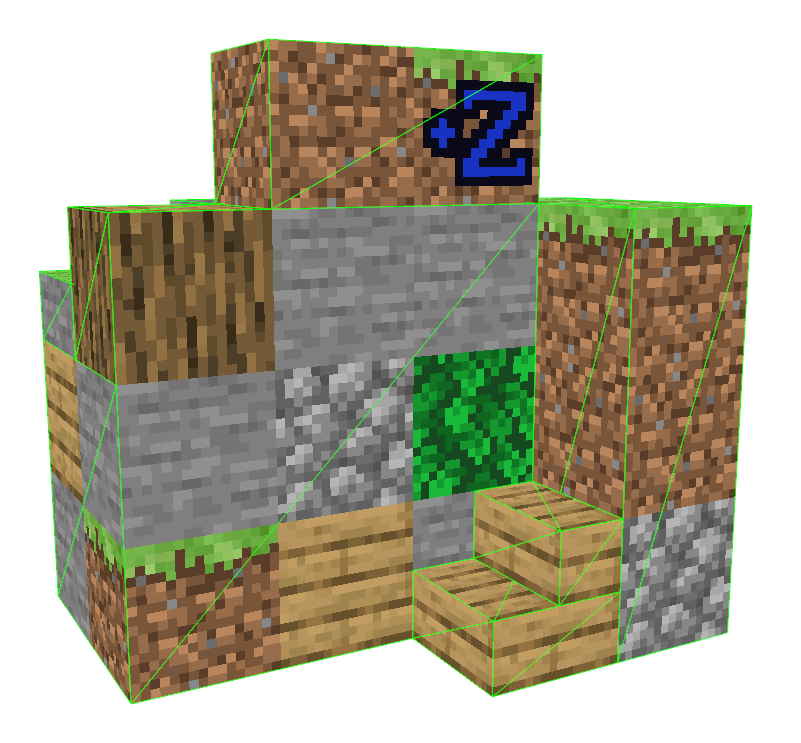
\includegraphics[width=0.5\textwidth]{../assets/greedy/many_textures.png}
\end{center}
